\documentclass[tikz,border=0pt,crop=true]{standalone}

\usepackage{tikz} % Allows creation of tikz pictures
\usepackage{varwidth}
\usetikzlibrary{arrows,shapes}

\begin{document}
    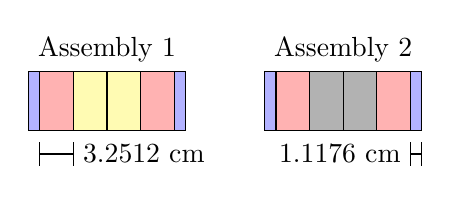
\begin{tikzpicture}[scale=1.0, every node/.style={scale=1}]
        % Draw water boxes
        \foreach \x in {0.0, 1.853333333, 3.0, 4.853333333}
        \filldraw[xshift=\x cm,fill=blue!30!white,draw=black] (0,0) 
        rectangle (0.14666666,0.75);
        % Draw uo2-1
        \foreach \x in {0.14666666, 1.426666666, 3.14666666, 4.426666666}
        \filldraw[xshift=\x cm,fill=red!30!white,draw=black] (0,0) 
        rectangle (0.42666667,0.75);
        % Draw uo2-2
        \foreach \x in {0.57333333, 1.0}
        \filldraw[xshift=\x cm,fill=yellow!30!white,draw=black] (0,0)
        rectangle (0.42666667,0.75);
        % Draw uo2-Gd
        \foreach \x in {3.57333333, 4.0}
        \filldraw[xshift=\x cm,fill=black!30!white,draw=black] (0,0)
        rectangle (0.42666667,0.75);
        \draw (1.0,0.75) node[above] {Assembly 1};%
        \draw (4.0,0.75) node[above] {Assembly 2};%
        \draw (4.853333333,-.15) -- (4.853333333,-.45) -- (4.853333333,-.30) node[left] {1.1176 cm} -- 
        (5.0,-.30) -- (5.0,-.15) -- (5.0, -.45);
        \draw (0.14666666,-.15) -- (0.14666666,-.45) -- (0.14666666,-.30) -- (0.57333333,-.30) node[right] {3.2512 cm} -- (0.57333333,-.15) -- (0.57333333, -.45);
    \end{tikzpicture}
\end{document}
